%===============================================================
% Template author: Martin Malý.
% Template URL: https://www.overleaf.com/latex/templates/czech-technical-university-colors-beamer-template-lab-of-structure-of-biomolecules/xmgmzfhtyrxt
%===============================================================

\documentclass{beamer}
% \documentclass[aspectratio=169]{beamer} % Uncomment for 16:9
\usepackage[utf8]{inputenc}

\usetheme{Madrid}

\definecolor{cvut_navy}{HTML}{0065BD}
\definecolor{cvut_blue}{HTML}{6AADE4}
\definecolor{cvut_gray}{HTML}{156570}

\setbeamercolor{section in toc}{fg=black,bg=white}
\setbeamercolor{alerted text}{fg=cvut_blue}
\setbeamercolor*{palette primary}{bg=cvut_navy,fg=gray!20!white}
\setbeamercolor*{palette secondary}{bg=cvut_blue,fg=white}
\setbeamercolor*{palette tertiary}{parent=palette primary}
\setbeamercolor*{palette quaternary}{fg=green,bg=gray!5!white}

\setbeamercolor*{sidebar}{fg=cvut_navy,bg=gray!15!white}


\setbeamercolor{titlelike}{parent=palette primary}
\setbeamercolor{frametitle}{parent=palette primary}

\setbeamercolor*{separation line}{}
\setbeamercolor*{fine separation line}{}

\setbeamertemplate{navigation symbols}{}

% Change itemize and enumerate style.
\setbeamertemplate{itemize item}{%
  \textcolor{cvut_navy}{\raisebox{.45ex}{\rule{.8ex}{.8ex}}}
}
\setbeamertemplate{enumerate item}{%
  \textcolor{cvut_navy}{\arabic{enumi}.}
}

\usepackage{eqnarray,amsmath}
\usepackage{amsfonts}
\usepackage{amssymb}
\usepackage{graphicx}
\usepackage{lmodern} % for bold and italic at the same time
\usepackage{bm} % for bold and italic at the same time
\usepackage{epstopdf}
\usepackage{changepage}
\usepackage{array,booktabs}
\usepackage[dua, nolist]{acronym}

%% | -------------------------- tikz -------------------------- |

\usepackage{tikz}
\usepackage{pgfplots}
\pgfplotsset{compat=1.14}
\usetikzlibrary{backgrounds,arrows,automata,shapes,positioning,calc,through,spy,shapes,shapes.geometric,shapes.multipart,fit,patterns,fadings}
\pgfdeclarelayer{background}
\pgfdeclarelayer{foreground}
\pgfsetlayers{background,main,foreground}


%====================================================
%========== DEFINITION OF AUTHORS ETC...=============
%====================================================
\author[Yauheni Zviazdou]{Yauheni Zviazdou}
\institute[CTU FEE]{Czech Technical University in Prague \\ Faculty of Electrical Engineering \\ Department of Cybernetics \\}
\title[Text representation models. RAG.]{From FastText to Transformer Models, and their Application in Retrieval-Augmented Generation}
\date[Bachelor's thesis presentation]{Bachelor's thesis presentation\\Supervisor: Ing. Jan Šedivý, CSc.}

%====================================================
%========== BEGINNING OF DOCUMENT ===================
%====================================================
\begin{document}


% Title slide
\begin{frame}
  \titlepage
  \begin{center}
    
\includegraphics[height=2cm]{src/fig/pdfs/ctu_logo_blue_filled.pdf}
  \end{center}
  %!TEX root = ../main.tex

\begin{acronym}
  \acro{CTU}[CTU]{Czech Technical University}
  \acro{API}[API]{Application Programming Interface}
  \acro{RAG}[RAG]{Retrieval-Augmented Generation}
  \acro{NLP}[NLP]{Natural Language Procession}
  \acro{STS}[STS]{Semantic Textual Similarity}
  \acro{QA}[QA]{Question Answering}
  \acro{BERT}[BERT]{Bidirectional Encoder Representations from Transformers}
  \acro{CBOW}[CBOW]{Continuous Bag-of-Words}
  \acro{GloVe}[GloVe]{Global vectors}
  \acro{ML}[ML]{Machine Learning}
  \acro{NN}[NN]{Neural Network}
  \acro{BoW}[BoW]{Bag-of-Words}
  \acro{TF-IDF}[TF-IDF]{Term Frequency-Inverse Document Frequency}
  \acro{OOV}[OOV]{Out of vocabulary}
\end{acronym}

\end{frame}

% Add CTU logo to the all slides excluding title
\logo{
\includegraphics[height=1cm]{src/fig/pdfs/ctu_logo_blue_filled.pdf}}


% Motivation
\begin{frame}
  \frametitle{Motivation}

\end{frame}

% Work objectives
\begin{frame}
  \frametitle{Work objectives}
  \textcolor{cvut_navy}{Task 1.} Compare text representation for QA\footnote{Question Answering}:
  \begin{itemize}
    \item Review text representation methods.
    \item Compare traditional and transformer-based methods.
  \end{itemize}
  \textcolor{cvut_navy}{Task 2.} RAG\footnote{Retrieval-Augmented Generation} Optimization
  \begin{itemize}
    \item Choose optimal models for RAG.
    \item Choose optimal chunk size and number of context chunks.
  \end{itemize}

\end{frame}

% Text representation
\begin{frame}
  \frametitle{Text representation}
\end{frame}


% Word embedding methods
\begin{frame}
  \frametitle{Word embedding methods}
\end{frame}

% Methods of text representations evaluation
\begin{frame}
  \frametitle{Word embedding methods}
\end{frame}

% Retrieval-Augmented Generation (RAG)
\begin{frame}
  \frametitle{Retrieval-Augmented Generation (RAG)}
  \begin{columns}[onlytextwidth,T]
    \begin{column}{0.75\textwidth}
      \begin{figure}[h]
        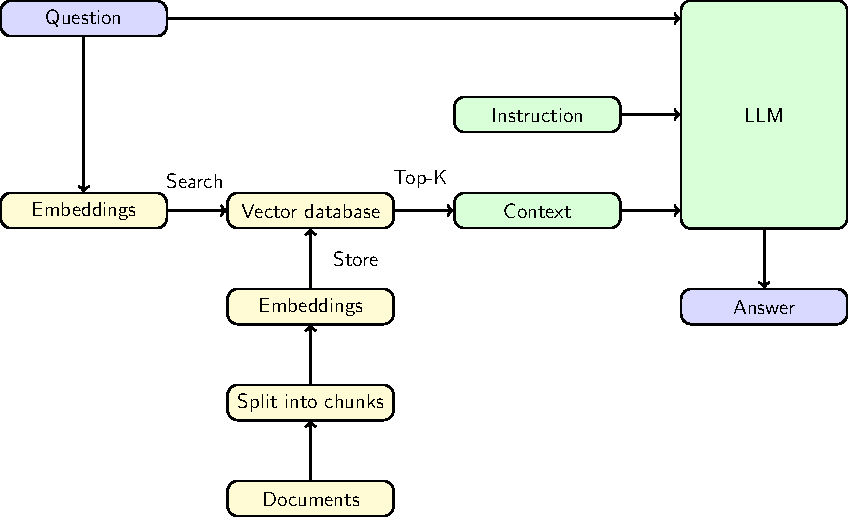
\includegraphics[scale=0.6]{src/fig/pdfs/tikz/RAG_scheme.pdf}
        \caption{Architecture of the RAG algorithm.}
       \end{figure}
    \end{column}

      \begin{column}{0.75\textwidth}
        Factors:  
        \begin{enumerate}
          \item Embedding \\model
          \item Chunk size
        \end{enumerate}
    \end{column}
  \end{columns}
  
  
\end{frame}

% Methodology
\begin{frame}
  \frametitle{Methodology}
\end{frame}

% Balanced models
\begin{frame}
  \frametitle{Balanced models}
\end{frame}

% Optimizing RAG
\begin{frame}
  \frametitle{Optimizing RAG}
\end{frame}

% Thanks
\begin{frame}
  \frametitle{Thanks}
\end{frame}

\begin{frame}
  \frametitle{Next slide}
  \begin{columns}[onlytextwidth]
    \begin{column}{0.5\textwidth}
      \begin{itemize}
        \item Text
        \item \textbf{Text}
          \item \textcolor{cvut_navy}{Text}
          \item \textcolor{cvut_navy}{\textbf{Text}}
      \end{itemize}
    \end{column}

      \begin{column}{0.5\textwidth}
       \begin{enumerate}
        \item Text
        \item \textbf{Text}
          \item \textcolor{cvut_navy}{Text}
          \item \textcolor{cvut_navy}{\textbf{Text}}
      \end{enumerate}
    \end{column}
  \end{columns}
\end{frame}


\end{document}
% =============================================================
% =========================== END =============================
% =============================================================

